\section{Представление геометрической информации в различных видах ПО}\label{sec:geoDifferentReprs}

% ================================================================================================================
%   ____    _    ____                                      _              
%  / ___|  / \  |  _ \      __ _  ___  ___  _ __ ___   ___| |_ _ __ _   _ 
% | |     / _ \ | | | |    / _` |/ _ \/ _ \| '_ ` _ \ / _ \ __| '__| | | |
% | |___ / ___ \| |_| |   | (_| |  __/ (_) | | | | | |  __/ |_| |  | |_| |
%  \____/_/   \_\____/     \__, |\___|\___/|_| |_| |_|\___|\__|_|   \__, |
%                          |___/                                    |___/ 
% ================================================================================================================

\subsection{Граничное представление BREP}\label{sec:geoCAD}

%Ссылка на Голованова должна появиться где-то
В BREP есть два типа понятий --- геометрические (<<точка>>, <<кривая>>, <<поверхность>>) и топологические (<<вершина>>, <<ребро>>, <<грань>>). <<Точка>> --- это тройка координат в некоторой системе координат. <<Кривая>> --- это уравнение, задающее множество точек, принадлежащих данной кривой. Кривую удобно описать с помощью параметрического уравнения от одной переменной. <<Поверхность>> --- это уравнение, задающее множество точек, принадлежащих данной поверхности. Соответственно, поверхность удобно описать с помощью параметрического уравнения от двух переменных. Топологические сущности задаются на базе геометрических. <<Вершина>> лежит в некоторой геометрической точке. <<Ребро>> лежит на некоторой геометрической кривой и ограничено двумя вершинами. Очевидно, что эти вершины должны принадлежать кривой, то есть и соответствующие геометрические точки должны принадлежать кривой. <<Грань>> лежит на некоторой поверхности и ограничена замкнутым циклом из рёбер. Также очевидно, что эти рёбра должны принадлежать поверхности, как и кривые, на которых они лежат, как и вершины и точки, ограничивающие эти рёбра. Замкнутая оболочка из граней с указанием внешних сторон этих граней ограничивает некоторую область пространства, называемую <<телом>>.

В памяти ЭВМ или обменном файле создаётся древовидная структура. Терминальными вершинами этого дерева чаще всего являются геометрические точки, представляющие собой тройки чисел с плавающей точкой. Далее вверх по дереву, имеются узлы типа вершина со ссылками на геометрические точки. Ребро также представляется в виде узла дерева, от которого идёт ссылка на геометрическую сущность, описывающую уравнение кривой, на которой это ребро построено, и ссылки на вершины, ограничивающие это ребро.

В соответствии с BREP параллелепипед (которому эквивалентен примитив box в CSG) задаётся следующим образом (\figref{fig:BREPbox1} и \figref{fig:BREPbox2}). На этих рисунках дерево представленно упрощённо. Имеется 8 вершин, каждое из 12 рёбер ограничено двумя из этих восьми вершин. Описание вершин не дублируется, на одну и у же сущность может быть множество ссылок. Аналогичным образом каждая из 6 граней ограничена прямоугольником --- циклом из четырёх рёбер, поэтому от каждой сущности типа грань идёт 4 ссылки на рёбра. Тело представляется как замнутая оболочка из поверхностей, поэтому от сущности типа solid идут ссылки на 6 граней. Фактически, помимо представленной на рисунках структуры, имеется ещё довольно-таки много дополнительной информации, без которой корректное и однозначение описание было бы невозможным, например, направления рёбер, направления обхода в цикле из рёбер, направления нормалей граней, уравнения кривых и поверхностей (в данном примере лишь неявно, т.к. используются базовые прямые линии и плоскости), и т.д.

\begin{figure}[H]
\centering
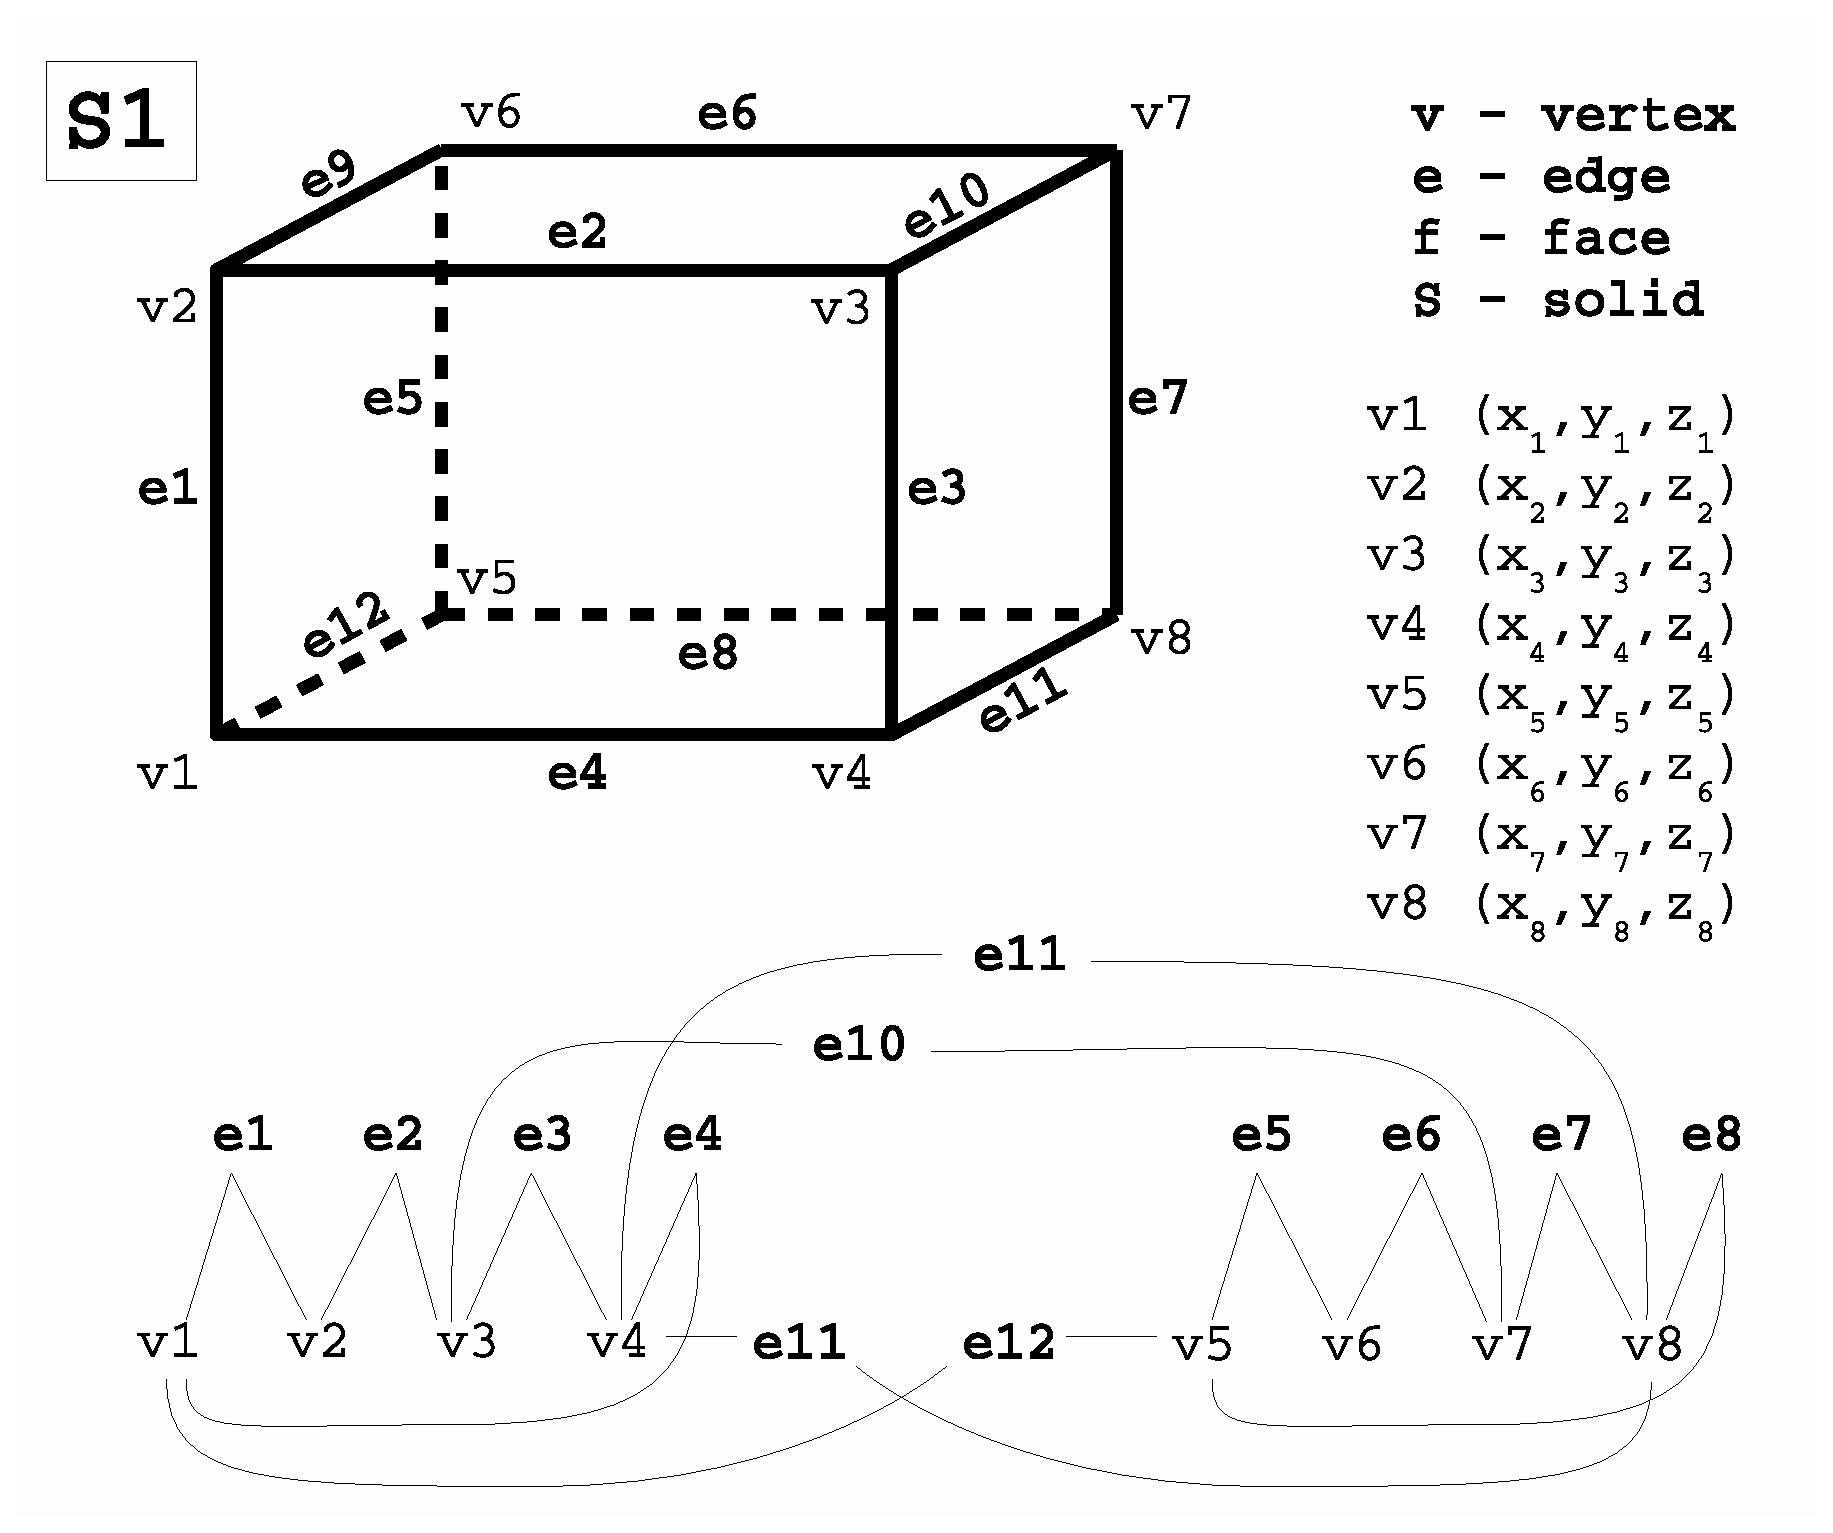
\includegraphics[width=0.7\textwidth]{pictures/BREPbox1.eps}
\caption{Описание вершин и рёбер примитива box методами BREP.}
\label{fig:BREPbox1}
\end{figure}

\begin{figure}[H]
\centering
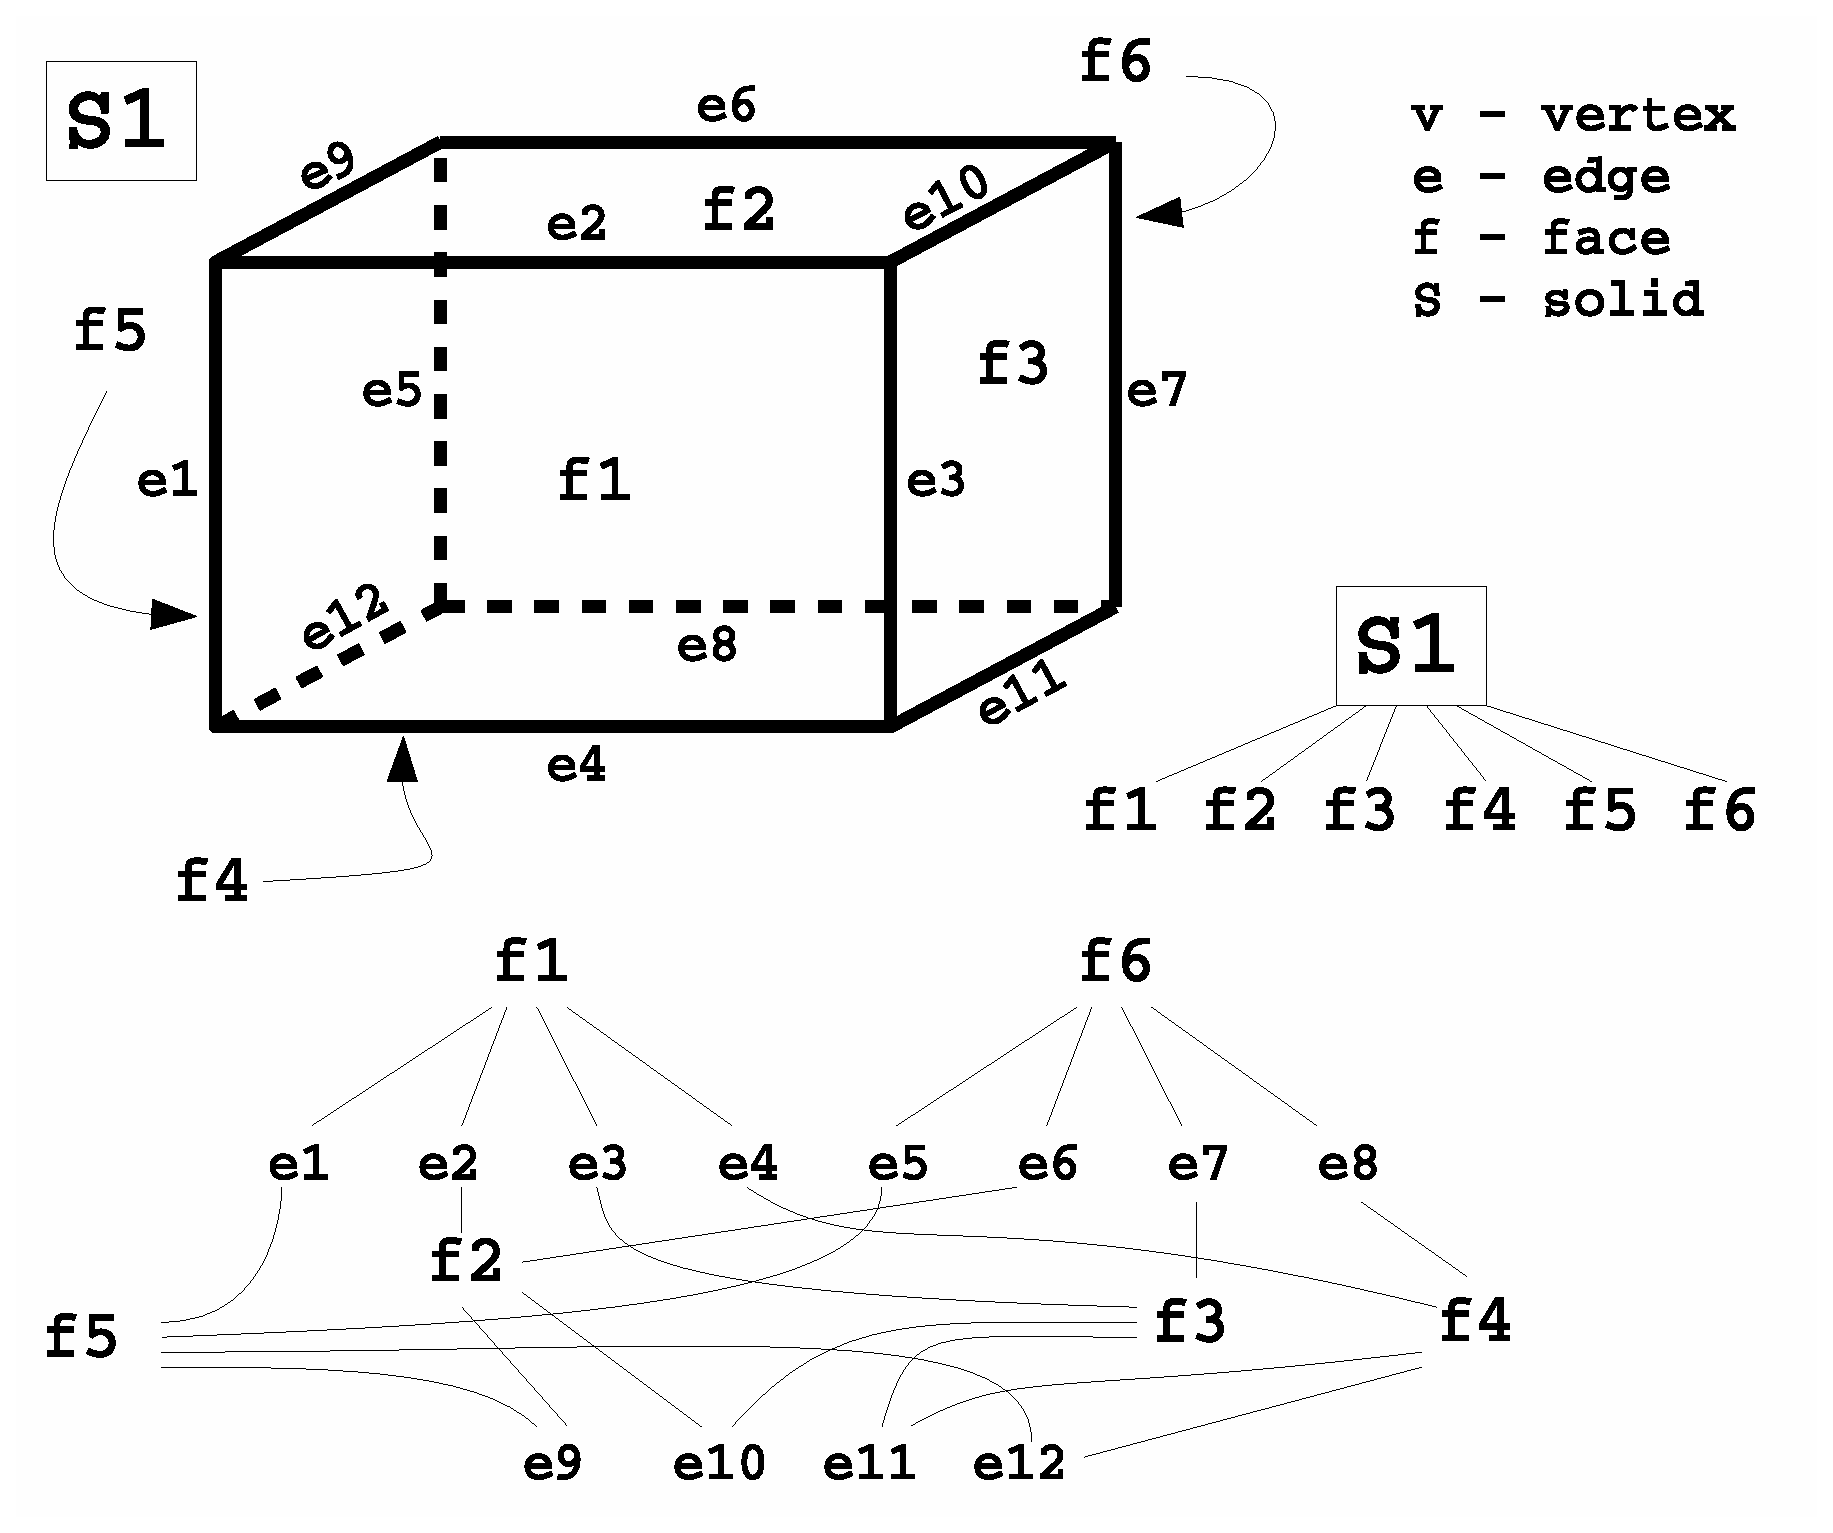
\includegraphics[width=0.7\textwidth]{pictures/BREPbox2.eps}
\caption{Описание граней и тела примитива box методами BREP.}
\label{fig:BREPbox2}
\end{figure}

Стоит, однако, отметить, что человек, создающий геометрическую модель в САПР, хотя и может выполнять построения в соответствии с базовыми принципами BREP, чаще всего применяет интуитивно понятные формообразования. Из последовательности этих формообразований система точно формирует BREP модель в памяти ЭВМ, которая также необходима для получения триангулированной геометрии для визуализации на дисплее ЭВМ~(\ref{sec:secGeoPoly}). Есть 4 базовых формообразования и 4 им обратных (с вычитанием) --- <<выдавливание>>, <<вращение>>, <<протягивание>> и <<тело по сечениям>>. Многие другие формообразования, такие как фаски и скругления, разрезы, отверстия, внутри на самом деле являются лишь вариациями перечисленных. Последовательность формообразований, выполненных пользователем для получения итоговой формы, сохраняется в виде дерева построения модели, напоминающего историю построения, но позволяющего навигацию и редактирование. Дерево часто доступно пользователю в основном рабочем окне интерфейса САПР. Однако бывают случаи, когда история построения теряется, например при передаче модели из одной САПР в другую. Таким образом, в результате работы инженера получается модель, описанная с помощью BREP, и во многих случаях имеющая также и дерево построения.

В инженерной практике принято проектировать и соответственно строить 3d-модели, объединяя в сборки детали и другие сборки. Отсюда вытекает, что во многих САПР, в том числе в CATIA~v5, существуют стандартные объекты, обозначающие детали и сборки. Например в САПР CATIA~v5 существует отдельный тип документа CATPart для детали и отдельный тип документа CATProduct для сборки. Внутри документа типа CATPart есть минимальный набор обязательных элементов --- 3 стандартные взаимноперпендикулярные плоскости в начале системы координат детали и главное тело детали, по умолчанию называемое PartBody. В документе типа CATProduct присутствует возможность добавлять в качестве дочерних компонентов либо документы CATPart либо другие документы CATProduct. В~\ref{sec:secBuilder} описывается, как соотносятся перечисленные сущности CATIA~v5 с понятиями геометрической подсистемы GEANT/ROOT.

Во многих САПР, в том числе и CATIA~v5 присутствует возможность так называемого контекстного редактирования компонентов. Это означает, что пользователь во время работы над сборкой в документе типа CATProduct, имеющей в качестве дочерних компонентов детали в файлах типа CATPart, может также редактировать эти детали, не переключая активный документ. Эта возможность широко используется в ``CATIA-GDML geometry builder'' --- большая часть работы выполняется в контексте единственного продукта, что с точки зрения пользователя аналогично работе над всей экспериментальной установкой.

\todo
Описать только нормальное применение BREP, то есть для замкнутых солидов.

% ================================================================================================================
%  _____ _____ __  __                                     _              
% |  ___| ____|  \/  |     __ _  ___  ___  _ __ ___   ___| |_ _ __ _   _ 
% | |_  |  _| | |\/| |    / _` |/ _ \/ _ \| '_ ` _ \ / _ \ __| '__| | | |
% |  _| | |___| |  | |   | (_| |  __/ (_) | | | | | |  __/ |_| |  | |_| |
% |_|   |_____|_|  |_|    \__, |\___|\___/|_| |_| |_|\___|\__|_|   \__, |
%                         |___/                                    |___/ 
% ================================================================================================================

\subsection{Конечно-элементное (КЭ) геометрическое представление}\label{sec:secGeoFEM}

\textbf{Повтор} \\
\textbf{Также, как и в любой другой прикладной области, необходимо выполнять многочисленные расчёты, которые нередко требуют геометрическую модель в качестве входных данных. Так, например, в инженерно-конструкторской среде широкое распространение получил метод конечных элементов (МКЭ) для решения задач прочности и устойчивости механических конструкций, динамики жидкостей и газов и т.д.}

Метод конечных элементов --- это численный метод решения дифференциальных уравнений с частными производными, а также интегральных уравнений, возникающих при решении задач прикладной физики. Метод широко используется для решения задач механики деформируемого твёрдого тела, теплообмена, гидродинамики и электродинамики.

Метод конечных элементов получил своё название от способа разбиения расчётной области на элементарные блоки --- конечные элементы (КЭ).
Строго говоря, КЭ --- это не только геометрическая форма, но и модель аппроксимации решения внутри области, ограниченной этой формой.
Существует огромное множество типов КЭ, причём существуют элементы имеющие одинаковую геометрию, но разные математические модели.
Расчётная область может быть разбита на элементы различных типов.
Исходя из условий решаемой задачи инженер-расчётчик выбирает, какими элементами разбивать расчётную область, а также, обычно, задаёт какие-либо указания модулю разбиения геометрии на сетку в расчётном программном обеспечении.
В простом случае расчётной областью является пространство заполненное материалом, т.е. сама деталь, а конечным элементом --- тетраэдр.
Модель, в которой деталь представлена множеством КЭ, соответственно называют КЭ-моделью.

\todo Картинка. Возможно, имеется смысл показать одну и ту же делать в разных геом. представлениях.

% Вырезан кусок... Ушёл в обмен геометриями

% ================================================================================================================
%   ____ ____   ____                                     _              
%  / ___/ ___| / ___|     __ _  ___  ___  _ __ ___   ___| |_ _ __ _   _ 
% | |   \___ \| |  _     / _` |/ _ \/ _ \| '_ ` _ \ / _ \ __| '__| | | |
% | |___ ___) | |_| |   | (_| |  __/ (_) | | | | | |  __/ |_| |  | |_| |
%  \____|____/ \____|    \__, |\___|\___/|_| |_| |_|\___|\__|_|   \__, |
%                        |___/                                    |___/ 
% ================================================================================================================

\subsection{Конструктивная твердотельная геометрия CSG}\label{sec:secGeoCSG}

В качестве строительных блоков в CSG используются примитивы из списка реализованных в системе. Список примитивов включает в себя как относительно простые примитивы типа параллелипипеда (box), сегмента цилиндра (tubs), сегмента конуса (cons), так и достаточно сложные, типа эллипсоида, параболоида, скрученных (twisted) примитивов. Принимая во внимание тот факт, что геометрия в GEANT/ROOT нужна для выполнения моделирования взаимодействия частиц с материалом, можно сказать, что примитив --- это объект, имеющий геометрическое представление и для которого реализовано решение геометрических задач, возникающих при моделировании. Среди таких геометрических задач можно отметить задачу нахождения расстояния до ближайшей границы примитива от некоторой точки внутри объёма, в одном заданном направлении или в любом возможном направлении. Эту задачу необходимо решать многократно в процессе проведения частицы для того чтобы определить так называемый максимальный допустимый геометрический шаг. В результате моделирования физических процессов получается максимальный допустимый шаг из соображений физики. Для того чтобы собственно изменить координату частицы из этих двух шагов выбирается минимальный. Каждый примитив, как в GEANT4, так и в ROOT, реализован как отдельный C++ класс, имеющий свои геометрические параметры среди членов данных, и решение описанных выше геометрических задач среди методов. Следует, отметить, что есть только параметры примитива, но нет никакого описания типа BREP. Уравнения границ фигурируют лишь в неявном виде в коде методов для решения геометрических задач. Более подробно примитивы описаны в~\ref{sec:Primitives}.

Форма может быть описана как результат Булевой операции над примитивами или другими Булевыми операциями. Есть три Булевы операции --- объединение (union), вычитание (subtraction) и пересечение (intersection). Булевы операции позволяют задать практически любую геометрическую форму, имеющую границы из тех, что применяются в примитивах. При этом не требуется дополнительной реализации решения геометрических задач, т.к. удаётся комбинировать то, что реализовано в примитивах. Более подробно применение Булевых операций для задания формы объёма описано в~\ref{sec:Boolean}.

Изначально CSG использовался как основной способ представления геометрии в САПР, но по мере развития последних от CSG перешли к BREP. При этом, всё же, во многих САПР осталась возможность создавать CSG геометрию.
CSG до сих пор активно применяется для описания ячейки периодичности композитных материалов.

\todo NEU, ANEU

% ================================================================================================================
%  ____       _                               _                                     _              
% |  _ \ ___ | |_   _  __ _  ___  _ __   __ _| |     __ _  ___  ___  _ __ ___   ___| |_ _ __ _   _ 
% | |_) / _ \| | | | |/ _` |/ _ \| '_ \ / _` | |    / _` |/ _ \/ _ \| '_ ` _ \ / _ \ __| '__| | | |
% |  __/ (_) | | |_| | (_| | (_) | | | | (_| | |   | (_| |  __/ (_) | | | | | |  __/ |_| |  | |_| |
% |_|   \___/|_|\__, |\__, |\___/|_| |_|\__,_|_|    \__, |\___|\___/|_| |_| |_|\___|\__|_|   \__, |
%               |___/ |___/                         |___/                                    |___/ 
% ================================================================================================================

\subsection{Полигональное геометрическое представление}\label{sec:secGeoPoly}

Полигональное (тесселированное, фасеточное) представление не менее распростанено, но имеет совершенно другую область применения. Строительным элементом полигональных моделей в общем случае является плоский многоугольник, называемый полигоном (polygon, pgon) или фасеткой (facet). Несколько таких многоугольников может стыковаться по рёбрам или вершинам, образуя поверхность, возможно описывающую границы некоторого объекта. Из этого следует, что, строго говоря, полигональное представление является частным случаем BREP с некоторыми допущениями, однако принято рассматривать его как отдельный способ по нескольким причинам.

Для моделирования прохождения частиц через геометрию для каждого объёма обязательно должны быть определены его границы, отделяющие материал этого объёма от окружающего пространства. Аналогично, для моделирования с помощью МКЭ (например, задач напряжённо-деформированного состояния) также необходимо точно задать геометрические границы деталей, для того чтобы указать материал внутри этих границ. Объект полигональной модели в общем случае не обязан быть замкнутым. Это означает, что, в принципе, между полигонами могут быть зазоры. Это объясняется тем, что полигональные модели изначально рассчитаны на быструю визуализацию, а не выполнение над ними каких-либо расчётов.

Полигональная геометрия в основном применяется в мультипликации, для получения фотореалистичных изображений. При этом основное внимание уделяется не математически точному описанию границ поверхностей, а реалистичности или художественности визуализации модели на дисплее.
%В общем случае такая модель не требует наличия замкнутой оболочки для задания тела, допускается даже остсутствие части границ, если это не влияет на изображение на экране.
Для создания и удобного редактирования полигональных моделей применяется соответствующее ПО: Autodesk 3ds Max, Autodesk Maya, Blender и др.

Частный случай полигонального представления --- триангулированное представление --- имеет треугольники в качестве полигонов. Оно представляет особый интерес т.к. всегда строится для визуализизации на дисплее графической подсистемой того или иного пакета моделирования, даже если пользователь создаёт BREP или CSG. Главная причина для этого заключается в том, что триангулированные модели могут очень быстро обрабатываться 3D-конвейером графического адаптера ПК, как наиболее важный частный случай --- визуализироваться на дисплее.

% http://elanina.narod.ru/lanina/ind/graph/file103.htm

Большинство приложений трёхмерной графики, в том числе САПР, при построении объемных сцен придерживаются определенной последо­вательности действий, в совокупности составляющей так называемый ЗD-конвейер. В качестве входных данных 3D-конвейер принимает массив треугольников, а итогом работы ЗD-конвейера является отрисовка (рендеринг) резуль­тирующего изображения на дисплее компьютера. Графический адаптер реализует аппаратное ускорение 3D-конвейера.

%OpenGL (Open Graphics Library) --- спецификация, определяющая платформонезависимый (независимый от языка программирования) программный интерфейс для написания приложений, использующих двумерную и трёхмерную компьютерную графику. OpenGL де-факто является стандартом для всех трёхмерных приложений, его конвейер представлен на~\figref{fig:OGLpipeline}.

%\begin{figure}[H]
%\includegraphics[width=0.8\textwidth]{pictures/pipeline-v4.png}
%\caption{Упрощённый конвейер OpenGL. На вход поступают координаты вершин и тройки индексов вершин, образующие треугольник. Выходной результат --- растровое (пиксельное) изображение, пригодное для отображения на дисплее.}
%\label{fig:OGLpipeline}
%\end{figure}

В промышленном геометрическом моделировании триангулированная геометрия применяется не только для визуализации. Например в стереолитографии, и вообще прототипировании, получил распространение формат обмена триангулированной геометрией STL, представляющий собой текстовый файл, в котором перечислены треугольники как группы по три вершины, а вершина задаётся тройкой координат (см. секцию~\ref{sec:secSTL}).

% ================================================================================================================
%   ____                 __                            _       
%  / ___| ___  ___      / _| ___  _ __ _ __ ___   __ _| |_ ___ 
% | |  _ / _ \/ _ \    | |_ / _ \| '__| '_ ` _ \ / _` | __/ __|
% | |_| |  __/ (_) |   |  _| (_) | |  | | | | | | (_| | |_\__ \
%  \____|\___|\___/    |_|  \___/|_|  |_| |_| |_|\__,_|\__|___/
%                                                              
% ================================================================================================================

\subsection{Обмен геометрической информацией}\label{sec:secGeoFormats}

Существует огромное множество форматов для обмена геометрией между различными программными продуктами. Следует различать геометрическое представление и формат, в котором данные записаны в файл. Существуют универсальные форматы, которые позволяют записывать в файл геометрию, представленную разными способами (например, BREP и триангулированная), но в большинстве случаев один формат подразумевает один способ представления геометрии. Данные могут быть записаны в файл как в виде текста, так и  бинарном виде. Проприетарные форматы в большинстве своём не имеют открытой спецификации, поэтому файлы этого формата бинарные, создаются и читаются только программами, имеющими 
, чаще всего разработанными фирмами, являющимися авторами этих форматов.
Можно купить лицензию на модуль импорта/экспорта и припилить к своей проге.
% \todo причесать.

\subsubsection{STEP}\label{sec:secSTEP}

В инженерной практике для обмена информацией об изделии, в том числе геометрическими моделями, наибольшее распространение получил независимый стандарт ISO-10303 STEP (STandard for Exchange of Product model data). (\todo В наши дни) Практически любая САПР имеет возможность импорта и экспорта STEP.
Данный стандарт предоставляет широкие возможности по обмену геометрией, однако его особенностью является наличие большого количества инструментов для описания геометрии, представленной в виде BREP.
% \todo расширить, пояснить

Обменные файлы STEP являются текстовыми. С одной стороны, это значительно упрощает разработку модулей для их импорта и экспорта. С другой стороны, это приводит к тому, что размер таких файлов становится достаточно большим для крупных моделей, а следовательно и растёт их время обработки.

\subsubsection{STL}\label{sec:secSTL}

STL (STereoLithography) --- текстовый формат для обмена тесселированной геометрией, который, возможно, является самым распространённым на данный момент форматом для передачи моделей в сфере 3d-сканирования и 3d-печати.

\subsubsection{CGR}\label{sec:secCGR}

% http://www.datakit.com/en/news/who-or-what-is-cgr--92.html

CGR (Catia Graphical Representation) --- проприетарный формат Dassault Systemes, используемый для хранения триангулированной модели, готовой для быстрой визуализации на дисплее.
Позволяет одновременно, в одном файле, хранить несколько моделей, что широко применяется для хранения нескольких уровней детализации.
% \todo проверить

\subsubsection{OBJ}\label{sec:secOBJ}

OBJ --- очень простой и открытый текстовый формат для обмена полигональными моделями. В файл OBJ записаны координаты вершин, списки индексов вершин каждого полигона и некоторые вспомогательные данные, типа текстурных координат и др.

\subsubsection{VRML, WRL, X3D}\label{sec:secVRML}

VRML (Virtual Reality Modeling Language) \\
WRL --- расширение файла \\
Наследник --- X3D.

\subsubsection{COLLADA}\label{sec:secCOLLADA}

% https://www.iso.org/standard/59902.html
% https://en.wikipedia.org/wiki/COLLADA
% https://www.khronos.org/collada/

Основанный на XML формат COLLADA (COLLAborative Design Activity) разработан специально для обмена геометрической информацией между интерактивными приложениями, такими как игровые движки, различные системы полигонального моделирования, САПР, и т.д. Файлы формата COLLADA имеют расширение dae (digital asset exchange). Формат COLLADA поддерживается некоммерческой организацией Khronos group, а в 2013 году был опубликован как международный стандарт ISO/PAS 17506:2012.

% ================================================================================================================
%     _         _                                               _             
%    / \  _   _| |_ ___        ___ ___  _ ____   _____ _ __ ___(_) ___  _ __  
%   / _ \| | | | __/ _ \      / __/ _ \| '_ \ \ / / _ \ '__/ __| |/ _ \| '_ \ 
%  / ___ \ |_| | || (_) |    | (_| (_) | | | \ V /  __/ |  \__ \ | (_) | | | |
% /_/   \_\__,_|\__\___(_)    \___\___/|_| |_|\_/ \___|_|  |___/_|\___/|_| |_|
%                                                                             
% ================================================================================================================

\subsection{Возможности автоматического перевода между способами представления}\label{sec:secAutoConversion}

\subsubsection{Конвертация CSG в BREP}\label{sec:secCSGtoBREP}

Поверхности, используемые в качестве границ примитивов CSG --- это чаще всего поверхности, описываемые относительно простыми уравнениями; большая часть из них --- уравнения первого и второго порядка. Очевидно, что перевод отдельных примитивов в BREP-описание не представляет сложности независимо от вида уравнений, описывающих их границы --- для этого не требуется никаких дополнительных вычислений. Чуть более сложная задача, но всё же полность решённая, --- автоматический перевод формы, полученной в результате Булевой операции, в BREP-описание. В случае Булевой операции в CSG нет явного описания рёбер и вершин, полученных в результате пересечения отдельных граней примитивов, однако эти рёбра вершины напрямую получаются из параметров операндов и их позиционирования. Таким образом возможна полная и \todo беспроблемная \todo конвертация CSG-модели в BREP, и она реализована, возможно в неявном виде, во всех САПР.

\subsubsection{Конвертация BREP в Polygonal}\label{sec:secBREPtoPolygonal}

Суть получения полигональной геометрии из полноценного BREP описания заключается в аппроксимации всех граней набором плоских фасеток. Очевидно, что если исходная грань не плоская, то аппроксиммирующая полиногальная сетка будет иметь от неё некоторое отклонение.
Давно разработаны и хорошо отлажены алгоритмы для такой аппроксимации. Точность аппроксимации --- управляющий параметр процедуры. Для более точной аппроксимации требуется больше полиногов, а следовательно возрастает нагрузка на графический адаптер
Многие из них основаны на триангуляции Делоне, разработанной в начале 20~века.

Таким образом возможна полная и \todo беспроблемная \todo конвертация BREP-модели в полигональную, и она реализована, возможно в неявном виде, во всех САПР.

\subsubsection{Конвертация BREP в FEM}\label{sec:secBREPtoFEM}

Существуют алгоритмы, позволяющие эффективно получить разбиение исходной геометрической модели, например представленной с помощью BREP и построенной в САПР, на конечные элементы. Из того что возможен автоматический перевод из CSG в BREP вытекает, что возможен также и перевод из CSG в КЭ-модель.

Первый этап процедуры разбиения твёрдого тела на конечные элементы заключается в триангуляции и выполняется теми же алгоритмами, что и для получения полиногальных моделей из BREP. Затем на основе разбиения граней строится пространственная сетка.

\subsubsection{Конвертация из BREP в CSG}\label{sec:secBREPtoCSG}

Если тело (solid) представляет собой примитив, описанный средствами BREP (см. секцию~\ref{sec:geoCAD}), то представляется возможным реализовать алгоритм, распознающий этот факт и определяющий параметры примитива. Сначала необходимо выполнить проверку топологии тела (тело ограничено шестью плоскими гранями, стыкующимися по 12 рёбрам, и т.д.), затем выполнить геометрические проверки (перпендикурярность плоскостей, углы между рёбрами и т.д.). Задача усложнена тем, что за счёт богатых возможностей BREP фактически правильная фигура может быть описана бесконечным количеством способов. Можно привести следующий простой пример. Плоская прямоугольная грань может быть описана уравнением плоскости и замкнутым циклом из 4-х взаимноперпендикулярных рёбер (прямоугольник) на этой плоскости, а может быть разбита на два треугольника на той же плоскости, смежных по гипотенузе. Эти два описания обозначают геометрически эквивалентные формы, но во втором случае потребуется дополнительная процедура приведения двух треугольников к одному прямоугольнику --- суть, минимальному полному описанию.

\todo
не всякая пов-то бреп может быть описана границей примитива

Описанные выше геометрические задачи также имеют следующую особенность. По причине ограниченности машинного слова числа с плавающей запятой хранятся в ПК с ограниченной точностью и выполнение расчётов, включающих матричные преобразования и тригонометрические функции, приводят к появлению заметных вычислительных ошибок. В большинстве случаев удаётся преодолеть эту проблему округлением до заданного знака, т.к. на практике в компьютерном геометрическом моделировании можно задаться физически обоснованным пределом снизу, например 1~мкм, или, с запасом, 1~нм, т.е. заведомо на много порядков выше точности вычислений.
Но, к сожалению, это не всегда помогает.

К сожалению, в подавляющем большинстве случаев форма тела не является примитивом, поэтому требуется каким-то образом представить её как результат Булевой операции.

\subsubsection{Конвертация FEM в BREP}\label{sec:secFEMtoBREP}

На практике не возникает необходимости переводить описание модели из КЭ в какое-либо другое. КЭ-модель всегда (кроме каких-то экстренных ситуаций) получена построением сетки на основе BREP или CSG.
В КЭ-моделях границы тел описываются так же как и в полигональных. Следовательно, с теоретической точки зрения, перевод из FEM в BREP эквивалентен переводу из полигонального представления в BREP.

\subsubsection{Конвертация Polygonal в BREP}\label{sec:secPolyToBREP}

Данная задача возникает при обработке результатов 3d-сканирования.
Проблема имеет некоторое сходство с конвертацией CSG в BREP.




% ================================================================================================================
%   ____ _____    _    _   _ _____  ______   ___   ___ _____                                     _              
%  / ___| ____|  / \  | \ | |_   _|/ /  _ \ / _ \ / _ \_   _|     __ _  ___  ___  _ __ ___   ___| |_ _ __ _   _ 
% | |  _|  _|   / _ \ |  \| | | | / /| |_) | | | | | | || |      / _` |/ _ \/ _ \| '_ ` _ \ / _ \ __| '__| | | |
% | |_| | |___ / ___ \| |\  | | |/ / |  _ <| |_| | |_| || |     | (_| |  __/ (_) | | | | | |  __/ |_| |  | |_| |
%  \____|_____/_/   \_\_| \_| |_/_/  |_| \_\\___/ \___/ |_|      \__, |\___|\___/|_| |_| |_|\___|\__|_|   \__, |
%                                                                |___/                                    |___/ 
% ================================================================================================================

\section{Представление геометрии в GEANT/ROOT}\label{sec:secGeoROOT}

Для описания геометрических форм в пакетах GEANT/ROOT применяется CSG (см. секцию~\ref{sec:secGeoCSG}).

%Таким образом
Наблюдается некоторая аналогия между BREP и CSG, заключающаяся в том, что в любом случае сложное тело или базовый примитив имеет некоторые границы, заданные аналитическими выражениями. Корни этой аналогии лежат в фундаментальной математике. Однако решающая разница заключается в том, что для примитива эти границы чётко определены и имеется лишь ограниченное число параметров, позволяющих изменять форму примитива.

Вторая составляющая геометрического представления в GEANT/ROOT это иерархия объёмов. Введём понятия логического и физического объёмов, формы и материала. Логический объём, или просто объём это базовый элемент для построения иерархии объёмов. Объём описывает непозиционированный объект и всё, что находится внутри него. Объём характеризуется формой и материалом. Форма --- это заданные с помощью CSG границы пространства, по методу, описанному выше. Материал включает в себя описание химического состава, плотности, и т.д. При помещении одного логического объёма в другой, например объёма $A$ в объём $B$, образуется так называемый физический объём, или узел, $B_1$, который обозначается взаимоотношение $A$ и $B$ как материнский-дочерний и характеризуется некоторой матрицей позиционирования $B$ внутри $A$.

% упомянуть FLUKA

Существует несколько способов задать геометрию для GEANT/ROOT --- с помощью текста (geo), GDML, макрос на языке ``C'' для ROOT,...

% ================================================================================================================
%   ____ ____  __  __ _     
%  / ___|  _ \|  \/  | |    
% | |  _| | | | |\/| | |    
% | |_| | |_| | |  | | |___ 
%  \____|____/|_|  |_|_____|
%                           
% ================================================================================================================

\subsection{Geometry Description Markup Language (GDML)}\label{sec:secGDML}

В дополнение к форматам, перечисленным в секции~\ref{sec:secGeoFormats}.

%Ссылка на сайт
Язык разметки GDML разработан специально для обмена моделями представленными с помощью CSG с иерархией объёмов. GDML --- это XML-подобный язык. Файл на GDML имеет следующую структуру. Тэг верхнего уровня <gdml>, в нём 5 разделов:
\begin{enumerate}
\item <define>
\item <materials>
\item <solids>
\item <structure>
\item <setup>
\end{enumerate}

В секции <define> объявлены объекты, которые могут многократно использоваться в другой секции.
\begin{enumerate}
\item constant
\item quantity
\item variable
\item position
\item rotation
\item scale
\item matrix
\end{enumerate}
Все объекты должны иметь уникальные имена, определённые в значении аттрибута name. При работе с ``Builder'' используются лишь некоторые из перечисленных типов: variable, position, rotation. В ``Builder'' введено три объекта, которые всегда создаются в <define> секции: нулевой поворот ``identity'', нулевой сдвиг ``central'' и константа DEGtoRAD для перевода из градусов в радианы.

Секция <materials> предназначена для определения материалов, которые будут использоваться в модели. При описании логического объёма в секции <structure> должна быть ссылка на соответствующий тег <material> в секции <materials>. Стандартное применение GDML подразумевает, что в файле имеется полная информация о модели, в том числе и о материалах. Это означает, что при импорте GDML файла в GEANT4 или ROOT описание материалов будет взято из секции <materials>. На практике это оказывается очень неудобным, поэтому в экспериментальных пакетах, как например в CbmRoot, по умолчанию включена опция считывания из GDML только имена материала, игнорируя собственно описание. Однако в любом случае, для того чтобы GDML файл считался корректным с формальной точки зрения, для каждой ссылки должен существовать объект, на который эта ссылка указывает. В ``Builder'' мы используем минимальное dummy \todo описание, чтобы соблюсти правила XML файла, а фактически используется внешняя база материалов.

В секции <solids> приведено описание форм логических объёмов. Как и в случае с материалами, в секции <structure>, при описании логического объёма должна быть приведена сслыка на соответствующий тег в секции <solids>.

Секция <structure> --- обычно самая большая секция, в которой описываются логические объёмы и их иерархия. Тег <volume> имеет как минимум два дочерних тега --- ссылка на материал <materialref> с аттрибутом ref, имеющим в качестве значения имя материала, определённого в секции <materials>, и ссылка на форму объёма <solidref> с аттрибутом ref, имещим в качестве значения имя формы, определённой в секции <solids>. Помимо этих двух обязательных дочерних тегов могу присутствовать другие теги, описывающие внутренний состав логического объёма. Самый распространённый случай --- тег <physvol>, обозначающий дочерний объём и имеющий аттрибут ref, указывающий на определённое ранее описание другого объёма.

Последняя секция <setup> служит для объявления одного логического объёма в качестве объёма верхнего уровня. Также здесь задаётся название установки, которое в CbmRoot должно быть FairGeom.

% ================================================================================================================
%   ____    _    ____                      __  __  ____ 
%  / ___|  / \  |  _ \    __   _____      |  \/  |/ ___|
% | |     / _ \ | | | |   \ \ / / __|     | |\/| | |    
% | |___ / ___ \| |_| |    \ V /\__ \_    | |  | | |___ 
%  \____/_/   \_\____/      \_/ |___(_)   |_|  |_|\____|
%                                                       
% ================================================================================================================

\section{Сравнение представления геометрии в GEANT/ROOT и САПР}\label{sec:secROOTvsCAD}

Разница между двумя способами описания геометрической информации в САПР и пакетах моделирования прохождения частиц через материал GEANT/ROOT заключается в двух пунктах. Во-первых, отличается способ задания геометрических форм. В САПР применяется граничное представление (BREP), для описания которого используются понятия типа <<поверхность>>, <<грань>>, <<ребро>>, <<кривая>>, и за которыми стоят соответствующие уравнения, описывающие эти объекты в пространстве. В GEANT/ROOT применяется конструктивная твердотельная геометрия (CSG), которая оперирует понятиями <<примитив>> и <<Булева операция>>. Очевидно, что и за этими объектами также стоят конкретные уравнения, описывающие кривые и поверхности, однако есть существенное различие описанное ниже. Во-вторых, отличается способ задания взаимоотношения форм в пространстве. В САПР, по аналогии с тем, как человек воспринимает окружающий мир, присутствует некоторое бесконечное окружающее пространство без материала, а все предметы находятся в этом пространстве. Невозможна такая ситуация, чтобы один объект находился внутри другого --- в таком случае подразумевается, что во втором есть соответствующая полость, освобождающая место под первый объект. При этом получается, что границы двух тел, стоящих рядом, совпадают, т.е происходит дублирование информации. \todo В силу математики это приводит к неприятным эффектам. \todo В GEANT/ROOT для описания взаимоотношения форм используется иерархия объёмов. Это объясняется тем, что такой метод более удобен для описания геометрии, где главной задачей является однозначное задание материала в каждой точке пространства. Вводится понятие объёма --- сущности, имеющей форму и материал. Из всех объёмов выбирается один, называемый объёмом верхнего уровня, а остальные помещены либо в него, либо в какой-то другой, формируя таким образом дерево объёмов. При этом не происходит дублирования границ и нет упомянутых выше эффектов.
